% Cleaned bilingual LaTeX from chunks/04_darwin.md.
% Compile with XeLaTeX or LuaLaTeX for Chinese text. Requires graphicx for preserved images.
\providecommand{\darwinpair}[2]{%
  \par\noindent{\small\textsf{EN}\quad #1}\par
  \noindent{\textsf{中}\quad #2}\par\medskip
}
\providecommand{\darwinimage}[2][]{%
  \begin{figure}[htbp]
  \centering
  \IfFileExists{../#2}{\includegraphics[#1]{../#2}}{%
    \IfFileExists{#2}{\includegraphics[#1]{#2}}{%
      \fbox{\parbox{0.82\linewidth}{\centering Missing image reference preserved:\\\texttt{#2}}}%
    }%
  }%
  \end{figure}
}

\darwinimage[width=0.72\linewidth]{images/5f8522bcc13764df00ac41eb9c256db35f9c3982afaeab440b049ff6ba14d2ff.jpg}
\darwinimage[width=0.72\linewidth]{images/04890d618174d03e224376ed406b2bf95249a4704840eb328a547de8c5b8d66a.jpg}
\darwinimage[width=0.72\linewidth]{images/298c02d16853568398e971ddca4f30f6ce8faa50bad1e7e8b79389d63480f4ed.jpg}

\section*{On the Origin of Species\\《物种起源》}
\begin{center}
Charles Darwin\\
查尔斯·达尔文
\end{center}

\subsection*{Chapter IV: Natural Selection\\第四章：自然选择}

\darwinpair
{Natural Selection—its power compared with man's selection—its power on characters of trifling importance—its power at all ages and on both sexes—Sexual Selection—On the generality of intercrosses between individuals of the same species—Circumstances favourable and unfavourable to Natural Selection, namely, intercrossing, isolation, number of individuals—Slow action—Extinction caused by Natural Selection—Divergence of Character, related to the diversity of inhabitants of any small area, and to naturalisation—Action of Natural Selection, through Divergence of Character and Extinction, on the descendants from a common parent—Explains the Grouping of all organic beings.}
{自然选择——它同人工选择相比的力量——它对极细微性状的作用——它在各个年龄和两性中的作用——性选择——同种个体之间杂交的普遍性——有利于和不利于自然选择的条件，即杂交、隔离和个体数量——缓慢的作用——自然选择所造成的灭绝——性状分歧，它同任何小区域内生物的多样性以及归化有关——自然选择通过性状分歧和灭绝，对共同祖先的后裔所发生的作用——解释一切生物的类群排列。}

\darwinpair
{How will the struggle for existence, discussed too briefly in the last chapter, act in regard to variation? Can the principle of selection, which we have seen is so potent in the hands of man, apply in nature? I think we shall see that it can act most effectually. Let it be borne in mind in what an endless number of strange peculiarities our domestic productions, and, in a lesser degree, those under nature, vary; and how strong the hereditary tendency is. Under domestication, it may be truly said that the whole organisation becomes in some degree plastic. Let it be borne in mind how infinitely complex and close-fitting are the mutual relations of all organic beings to each other and to their physical conditions of life. Can it, then, be thought improbable, seeing that variations useful to man have undoubtedly occurred, that other variations useful in some way to each being in the great and complex battle of life should sometimes occur in the course of thousands of generations? If such do occur, can we doubt, remembering that many more individuals are born than can possibly survive, that individuals having any advantage, however slight, over others would have the best chance of surviving and of procreating their kind? On the other hand, we may feel sure that any variation in the least degree injurious would be rigidly destroyed. This preservation of favourable variations and the rejection of injurious variations, I call Natural Selection. Variations neither useful nor injurious would not be affected by natural selection, and would be left a fluctuating element, as perhaps we see in the species called polymorphic.}
{上一章过于简略地讨论过的生存斗争，将怎样作用于变异呢？我们已经看到，选择原则在人的手中具有巨大力量；它能否应用于自然界呢？我想我们将会看到，它能够极其有效地发生作用。请记住，我们的家养生物，以及程度较低的自然状态下的生物，会在无穷无尽的奇特性状上发生变异；还要记住遗传倾向是多么强。在家养状态下，确实可以说整个机体在某种程度上都变得具有可塑性。再请记住，一切生物彼此之间以及它们同物理生活条件之间的相互关系，是何等无限复杂而又严密契合。那么，既然毫无疑问已经出现过对人有用的变异，难道在成千上万代的过程中，有时不会出现某些以某种方式有利于每一种生物在复杂生命大战中生存的变异吗？如果这类变异确会发生，那么，只要想到出生的个体远比可能存活的个体多，我们还能怀疑那些比其他个体具有任何优势、哪怕极其微小优势的个体，最有机会存活并繁殖其同类吗？另一方面，我们也可以确信，任何哪怕只有最轻微有害的变异，都会被严格消灭。保存有利变异、排斥有害变异，我称之为自然选择。既无益也无害的变异不会受到自然选择的影响，而会作为一种浮动因素保留下来，也许正如我们在所谓多型种中所见到的那样。}

\darwinpair
{We shall best understand the probable course of natural selection by taking the case of a country undergoing some physical change, for instance, of climate. The proportional numbers of its inhabitants would almost immediately undergo a change, and some species might become extinct. We may conclude, from what we have seen of the intimate and complex manner in which the inhabitants of each country are bound together, that any change in the numerical proportions of some of the inhabitants, independently of the change of climate itself, would most seriously affect many of the others. If the country were open on its borders, new forms would certainly immigrate, and this also would seriously disturb the relations of some of the former inhabitants. Let it be remembered how powerful the influence of a single introduced tree or mammal has been shown to be. But in the case of an island, or of a country partly surrounded by barriers, into which new and better adapted forms could not freely enter, we should then have places in the economy of nature which would assuredly be better filled up if some of the original inhabitants were in some manner modified; for, had the area been open to immigration, these same places would have been seized on by intruders. In such case, every slight modification which in the course of ages chanced to arise, and which in any way favoured the individuals of any of the species by better adapting them to their altered conditions, would tend to be preserved; and natural selection would thus have free scope for the work of improvement.}
{要最清楚地理解自然选择可能的进程，我们不妨设想一个国家正在经历某种物理变化，例如气候变化。它的生物居民在数量比例上几乎会立即发生改变，有些种还可能灭绝。我们已经看到，每个地区的生物居民以亲密而复杂的方式彼此联系；因此可以推断，某些居民数量比例的任何变化，即使撇开气候变化本身不论，也会极其严重地影响许多其他居民。如果这个地区的边界是开放的，新的类型必定会迁入，而这也会严重扰乱原有某些居民之间的关系。请记住，单单引入一种树木或一种哺乳动物，就已显示出何等强大的影响。可是，对于岛屿，或部分被障碍包围、使新的并且更适应的类型不能自由进入的地区来说，自然经济中就会有一些位置；倘若某些原有居民以某种方式被改造，这些位置必定会被更好地填补。因为如果该区域向移入开放，同样的位置就会被外来的入侵者占据。在这种情况下，漫长岁月中偶然发生的每一种轻微改变，只要能以任何方式有利于某一种个体，使它们更好地适应改变了的条件，就会倾向于被保存下来；自然选择由此便有充分余地去进行改进的工作。}

\darwinpair
{We have reason to believe, as stated in the first chapter, that a change in the conditions of life, by specially acting on the reproductive system, causes or increases variability; and in the foregoing case the conditions of life are supposed to have undergone a change, and this would manifestly be favourable to natural selection, by giving a better chance of profitable variations occurring; and unless profitable variations do occur, natural selection can do nothing. Not that, as I believe, any extreme amount of variability is necessary; as man can certainly produce great results by adding up in any given direction mere individual differences, so could Nature, but far more easily, from having incomparably longer time at her disposal. Nor do I believe that any great physical change, as of climate, or any unusual degree of isolation to check immigration, is actually necessary to produce new and unoccupied places for natural selection to fill up by modifying and improving some of the varying inhabitants. For as all the inhabitants of each country are struggling together with nicely balanced forces, extremely slight modifications in the structure or habits of one inhabitant would often give it an advantage over others; and still further modifications of the same kind would often still further increase the advantage. No country can be named in which all the native inhabitants are now so perfectly adapted to each other and to the physical conditions under which they live, that none of them could anyhow be improved; for in all countries, the natives have been so far conquered by naturalised productions that they have allowed foreigners to take firm possession of the land. And as foreigners have thus everywhere beaten some of the natives, we may safely conclude that the natives might have been modified with advantage, so as to have better resisted such intruders.}
{正如第一章所说，我们有理由相信，生活条件的改变由于特别作用于生殖系统，会引起或增加变异性；在上述例子中，我们假定生活条件已经改变，这显然有利于自然选择，因为它使有益变异的发生有更好的机会；而如果没有有益变异发生，自然选择便无能为力。并不是说，我认为必须有极大量的变异性；人能够仅仅把某一方向上的个体差异累加起来而确实产生巨大结果，自然也能如此，而且由于它拥有无可比拟地更长的时间，就更加容易。我也不认为必须有任何重大的物理变化，例如气候变化，或必须有任何异常程度的隔离来阻止迁入，才会产生新的、空缺的位置，供自然选择通过改造和改进某些变异中的居民来填补。因为每个地区的一切居民都以精细平衡的力量共同斗争，某一居民在构造或习性上的极其轻微改变，往往就会使它比其他居民占有优势；而同类的进一步改变，又往往会进一步增加这种优势。没有任何一个国家可以说，它的一切本地居民现在已经如此完美地彼此适应，并适应其所处的物理条件，以至于它们无论如何都不能再被改进；因为在所有国家，本地生物都已经在某种程度上被归化生物所征服，允许外来者牢固地占据土地。既然外来者在各处都曾击败某些本地生物，我们便可以稳妥地断定：本地生物本来可以有利地被改造，从而更好地抵抗这些入侵者。}

\darwinpair
{As man can produce and certainly has produced a great result by his methodical and unconscious means of selection, what may not nature effect? Man can act only on external and visible characters: nature cares nothing for appearances, except in so far as they may be useful to any being. She can act on every internal organ, on every shade of constitutional difference, on the whole machinery of life. Man selects only for his own good; Nature only for that of the being which she tends. Every selected character is fully exercised by her; and the being is placed under well-suited conditions of life. Man keeps the natives of many climates in the same country; he seldom exercises each selected character in some peculiar and fitting manner; he feeds a long- and a short-beaked pigeon on the same food; he does not exercise a long-backed or long-legged quadruped in any peculiar manner; he exposes sheep with long and short wool to the same climate. He does not allow the most vigorous males to struggle for the females. He does not rigidly destroy all inferior animals, but protects during each varying season, as far as lies in his power, all his productions. He often begins his selection by some half-monstrous form; or at least by some modification prominent enough to catch his eye, or to be plainly useful to him. Under nature, the slightest difference of structure or constitution may well turn the nicely-balanced scale in the struggle for life, and so be preserved. How fleeting are the wishes and efforts of man! how short his time! and consequently how poor will his products be, compared with those accumulated by nature during whole geological periods. Can we wonder, then, that nature's productions should be far “truer” in character than man's productions; that they should be infinitely better adapted to the most complex conditions of life, and should plainly bear the stamp of far higher workmanship?}
{既然人能够并且确实已经通过有计划的和无意识的选择方法产生巨大结果，那么自然又有什么不能做到呢？人只能作用于外部的、可见的性状；自然并不关心外表，除非外表对某种生物有用。自然能够作用于每一个内部器官，作用于体质差异的每一种细微层次，作用于整个生命机器。人只是为自己的利益而选择；自然只为它所照管的生物的利益而选择。每一种被选择的性状都由自然充分加以运用；生物也被置于适宜的生活条件之下。人把许多气候下的本地生物养在同一个国家；他很少以某种特殊而合适的方式锻炼每一种被选择的性状；他用同样的食物喂养长喙和短喙的鸽子；他并不以任何特殊方式锻炼长背或长腿的四足动物；他让长毛和短毛的绵羊暴露于同一种气候之下。他不允许最强健的雄性为争夺雌性而斗争。他并不严格消灭一切劣等动物，而是在每个变化的季节里尽其所能保护他的所有产物。他的选择往往从某种半畸形的类型开始；或至少从某种显著到足以引起他注意、或明显对他有用的改变开始。在自然状态下，构造或体质上最轻微的差异，完全可能在生存斗争中拨动那架精密平衡的天平，从而被保存下来。人的愿望和努力多么短暂！他的时间多么短促！因此，同自然在整个地质时期中累积起来的产物相比，人的产物将会何等贫弱。既然如此，自然的产物在性状上远比人的产物更“真实”，更能无限良好地适应最复杂的生活条件，并且明显带有远为高超的工艺印记，我们又有什么可惊奇的呢？}

\darwinpair
{It may be said that natural selection is daily and hourly scrutinising, throughout the world, every variation, even the slightest; rejecting that which is bad, preserving and adding up all that is good; silently and insensibly working, whenever and wherever opportunity offers, at the improvement of each organic being in relation to its organic and inorganic conditions of life. We see nothing of these slow changes in progress, until the hand of time has marked the long lapse of ages, and then so imperfect is our view into long past geological ages that we only see that the forms of life are now different from what they formerly were.}
{可以说，自然选择在全世界每时每刻都在审察每一个变异，哪怕最轻微的变异也不放过；它排斥坏的，保存并累加一切好的；只要机会出现，无论何时何地，它都在静默而不知不觉地工作，使每一种生物在同其有机和无机生活条件的关系中得到改进。我们看不见这些缓慢变化正在进行，直到时间之手标记出漫长岁月的流逝；而那时我们对于久远地质年代的观察又如此不完善，以至于只能看出现在的生命类型不同于从前。}

\darwinpair
{Although natural selection can act only through and for the good of each being, yet characters and structures which we are apt to consider as of very trifling importance may thus be acted on. When we see leaf-eating insects green, and bark-feeders mottled grey; the alpine ptarmigan white in winter, the red grouse the colour of heather, and the black grouse that of peaty earth, we must believe that these tints are of service to these birds and insects in preserving them from danger. Grouse, if not destroyed at some period of their lives, would increase in countless numbers; they are known to suffer largely from birds of prey; and hawks are guided by eyesight to their prey, so much so that on parts of the Continent persons are warned not to keep white pigeons, as being the most liable to destruction. Hence I can see no reason to doubt that natural selection might be most effective in giving the proper colour to each kind of grouse, and in keeping that colour, when once acquired, true and constant. Nor ought we to think that the occasional destruction of an animal of any particular colour would produce little effect: we should remember how essential it is in a flock of white sheep to destroy every lamb with the faintest trace of black. In plants the down on the fruit and the colour of the flesh are considered by botanists as characters of the most trifling importance: yet we hear from an excellent horticulturist, Downing, that in the United States smooth-skinned fruits suffer far more from a beetle, a curculio, than those with down; that purple plums suffer far more from a certain disease than yellow plums; whereas another disease attacks yellow-fleshed peaches far more than those with other coloured flesh. If, with all the aids of art, these slight differences make a great difference in cultivating the several varieties, assuredly, in a state of nature, where the trees would have to struggle with other trees and with a host of enemies, such differences would effectually settle which variety, whether a smooth or downy, a yellow- or purple-fleshed fruit, should succeed.}
{尽管自然选择只能通过并为了每一种生物的利益而发生作用，但我们容易认为极其微不足道的性状和构造，也可能因此受到作用。当我们看到食叶昆虫呈绿色，食树皮的昆虫呈斑驳的灰色；高山雷鸟冬季为白色，红松鸡呈石南花的颜色，黑松鸡呈泥炭土的颜色时，我们必须相信，这些色调有助于这些鸟类和昆虫免遭危险。松鸡若在生命的某个时期不被消灭，就会增加到不可计数；众所周知，它们大量遭受猛禽的危害；而鹰隼凭视觉寻找猎物，甚至在欧洲大陆的某些地方，人们会被告诫不要饲养白鸽，因为白鸽最容易被捕杀。因此，我看不出有什么理由怀疑，自然选择能够极其有效地赋予每一种松鸡以适当的颜色，并在这种颜色一经获得后，使它真实而恒定地保持下去。我们也不应以为偶尔消灭某种特定颜色的动物不会产生多大效果；我们应当记住，在一群白羊中，消灭每一只带有最轻微黑色痕迹的羔羊是多么必要。在植物中，果实上的茸毛和果肉的颜色被植物学家看作极其细微的性状；可是我们从杰出的园艺家唐宁那里听说，在美国，光滑果皮的果实比有茸毛的果实更容易遭受一种象甲危害；紫色李子比黄色李子更容易遭受某种病害；而另一种病害又比起其他颜色果肉的桃子，更容易侵袭黄肉桃。即使借助所有人工手段，这些细微差异在栽培若干品种时也会造成巨大差别；那么在自然状态下，树木必须同其他树木以及大批敌害斗争时，这些差异必定会有效决定哪一种品种能够成功，是光滑的还是有茸毛的果实，是黄色果肉还是紫色果肉的果实。}

\begin{center}
[\ldots]
\end{center}

\darwinpair
{Natural selection will modify the structure of the young in relation to the parent, and of the parent in relation to the young. In social animals it will adapt the structure of each individual for the benefit of the community, if each in consequence profits by the selected change. What natural selection cannot do is to modify the structure of one species, without giving it any advantage, for the good of another species; and though statements to this effect may be found in works of natural history, I cannot find one case which will bear investigation. A structure used only once in an animal's whole life, if of high importance to it, might be modified to any extent by natural selection; for instance, the great jaws possessed by certain insects, and used exclusively for opening the cocoon, or the hard tip to the beak of nestling birds, used for breaking the egg. It has been asserted that of the best short-beaked tumbler-pigeons more perish in the egg than are able to get out of it; so that fanciers assist in the act of hatching. Now, if nature had to make the beak of a full-grown pigeon very short for the bird's own advantage, the process of modification would be very slow, and there would be simultaneously the most rigorous selection of the young birds within the egg which had the most powerful and hardest beaks, for all with weak beaks would inevitably perish; or, more delicate and more easily broken shells might be selected, the thickness of the shell being known to vary like every other structure.}
{自然选择会改变幼体相对于亲体的构造，也会改变亲体相对于幼体的构造。在社会性动物中，如果每一个个体都因此从所选择的改变中获益，自然选择就会为了群体的利益而使每个个体的构造得到适应。自然选择所不能做的，是不赋予某一种任何优势，却为了另一种的利益而改变前一种的构造；尽管自然史著作中可以找到这类说法，我却找不到一个经得起考察的例子。某种构造即使在动物一生中只使用一次，只要对它极其重要，也可以经由自然选择被改变到任何程度；例如某些昆虫拥有的大颚，专门用于打开茧；又如雏鸟喙端的坚硬突起，用于破壳而出。有人断言，在最优良的短喙翻飞鸽中，死在卵内的比能出壳的还多；因此养鸽者会协助孵化。现在，如果自然为了成鸽本身的利益而不得不使鸽子的喙变得很短，改变过程将会非常缓慢；同时，卵内幼鸟中那些拥有最有力、最坚硬喙的个体会受到最严格的选择，因为喙软弱的个体必然死亡；或者，更薄、更容易破裂的蛋壳可能被选择，因为壳的厚度也同其他一切构造一样会发生变异。}

\subsection*{Sexual Selection\\性选择}

\darwinpair
{Inasmuch as peculiarities often appear under domestication in one sex and become hereditarily attached to that sex, the same fact probably occurs under nature; and if so, natural selection will be able to modify one sex in its functional relations to the other sex, or in relation to wholly different habits of life in the two sexes, as is sometimes the case with insects. And this leads me to say a few words on what I call Sexual Selection. This depends not on a struggle for existence, but on a struggle between the males for possession of the females; the result is not death to the unsuccessful competitor, but few or no offspring. Sexual selection is, therefore, less rigorous than natural selection. Generally, the most vigorous males, those which are best fitted for their places in nature, will leave most progeny. But in many cases victory will depend not on general vigour, but on having special weapons, confined to the male sex. A hornless stag or spurless cock would have a poor chance of leaving offspring. Sexual selection, by always allowing the victor to breed, might surely give indomitable courage, length to the spur, and strength to the wing to strike in the spurred leg, as well as the brutal cock-fighter, who knows well that he can improve his breed by careful selection of the best cocks. How low in the scale of nature this law of battle descends I know not; male alligators have been described as fighting, bellowing, and whirling round, like Indians in a war dance, for the possession of the females; male salmons have been seen fighting all day long; male stag-beetles often bear wounds from the huge mandibles of other males. The war is, perhaps, severest between the males of polygamous animals, and these seem oftenest provided with special weapons. The males of carnivorous animals are already well armed; though to them and to others, special means of defence may be given through means of sexual selection, as the mane to the lion, the shoulder-pad to the boar, and the hooked jaw to the male salmon; for the shield may be as important for victory as the sword or spear.}
{既然在家养状态下，特殊性状常常出现在某一性别中，并以遗传方式附着于这一性别，那么同样的事实大概也发生在自然状态下；如果是这样，自然选择就能够按照一性同另一性之间的功能关系来改变某一性，或者按照两性在生活习性上的完全不同来改变某一性，正如昆虫中有时所见的那样。这使我想谈几句我称为性选择的东西。性选择并不依赖于生存斗争，而依赖于雄性之间为占有雌性而进行的斗争；其结果并不是失败竞争者死亡，而是留下很少后代或没有后代。因此，性选择没有自然选择那样严酷。一般说来，最强健的雄性，即最适合其在自然中地位的雄性，会留下最多后裔。但在许多情况下，胜利并不取决于一般的强健，而取决于仅限于雄性的特殊武器。无角的雄鹿或无距的公鸡，留下后代的机会就很小。性选择总是让胜利者繁殖，当然能够赋予不可征服的勇气、增长鸡距，并增强翅膀击打带距腿部的力量；残酷的斗鸡者也深知，他能通过仔细选择最好的公鸡来改良自己的品种。我不知道这一战斗法则在自然阶梯中向下延伸到何等低级的地方；据描述，雄性短吻鳄会为了占有雌性而争斗、吼叫、旋转，像印第安人跳战舞一样；人们见过雄性鲑鱼整天争斗；雄性锹甲常带着其他雄性巨大上颚造成的伤痕。战争也许在多配偶动物的雄性之间最为激烈，而它们似乎也最常装备特殊武器。食肉动物的雄性本来已经武装良好；不过对它们以及其他动物来说，通过性选择仍可赋予特殊的防御手段，例如狮子的鬃毛、野猪的肩垫、雄鲑鱼的钩状颌；因为盾牌对于胜利可能同剑或矛一样重要。}

\darwinpair
{Amongst birds, the contest is often of a more peaceful character. All those who have attended to the subject believe that there is the severest rivalry between the males of many species to attract the females by singing. The rock-thrush of Guiana, birds of Paradise, and some others, congregate; and successive males display their gorgeous plumage and perform strange antics before the females, which, standing by as spectators, at last choose the most attractive partner. Those who have closely attended to birds in confinement well know that they often take individual preferences and dislikes: thus Sir R. Heron has described how one pied peacock was eminently attractive to all his hen birds. It may appear childish to attribute any effect to such apparently weak means: I cannot here enter on the details necessary to support this view; but if man can in a short time give elegant carriage and beauty to his bantams, according to his standard of beauty, I can see no good reason to doubt that female birds, by selecting during thousands of generations the most melodious or beautiful males according to their standard of beauty, might produce a marked effect. I strongly suspect that some well-known laws with respect to the plumage of male and female birds, in comparison with the plumage of the young, can be explained on the view of plumage having been chiefly modified by sexual selection, acting when the birds have come to the breeding age or during the breeding season; the modifications thus produced being inherited at corresponding ages or seasons, either by the males alone, or by the males and females; but I have not space here to enter on this subject.}
{在鸟类中，争斗常常具有较为和平的性质。凡是注意过这一问题的人都相信，许多种的雄鸟之间存在最激烈的竞争，以歌声吸引雌鸟。圭亚那的岩鸫、极乐鸟以及其他一些鸟类会聚集起来；一只只雄鸟依次在雌鸟面前展示华美的羽衣，表演奇异的动作；雌鸟则站在一旁观看，最后选择最有吸引力的伴侣。仔细观察过笼养鸟类的人都很清楚，它们往往有个体性的偏好和厌恶；例如 R. Heron 爵士曾描述过，一只花斑孔雀怎样对他所有雌孔雀都具有格外的吸引力。把任何效果归因于这种看似微弱的手段，或许显得幼稚；我在这里不能详述支持这一观点所需的细节。但是，如果人能够在短时间内按照自己的美的标准，赋予矮脚鸡以优雅姿态和美丽，那么我看不出有什么充分理由怀疑，雌鸟按照自己的美的标准，在成千上万代中选择歌声最悦耳或最美丽的雄鸟，也可能产生显著效果。我强烈怀疑，关于雌雄鸟羽衣同幼鸟羽衣相比较的一些众所周知的规律，可以用这种观点来解释：羽衣主要是由性选择所改变，而性选择在鸟类达到繁殖年龄或处于繁殖季节时发生作用；由此产生的改变在相应年龄或季节遗传下来，或仅由雄性遗传，或由雌雄双方遗传。不过我在这里没有篇幅深入讨论这一问题。}

\darwinpair
{Thus it is, as I believe, that when the males and females of any animal have the same general habits of life, but differ in structure, colour, or ornament, such differences have been mainly caused by sexual selection; that is, individual males have had, in successive generations, some slight advantage over other males in their weapons, means of defence, or charms; and have transmitted these advantages to their male offspring. Yet I would not wish to attribute all such sexual differences to this agency: for we see peculiarities arising and becoming attached to the male sex in our domestic animals, as the wattle in male carriers, horn-like protuberances in the cocks of certain fowls, \&c., which we cannot believe to be either useful to the males in battle or attractive to the females. We see analogous cases under nature; for instance, the tuft of hair on the breast of the turkey-cock, which can hardly be either useful or ornamental to this bird. Indeed, had the tuft appeared under domestication, it would have been called a monstrosity.}
{因此，我相信，当任何动物的雌雄具有相同的一般生活习性，却在构造、颜色或装饰上有所不同，这类差异主要是由性选择造成的；也就是说，在连续世代中，个别雄性在武器、防御手段或魅力方面比其他雄性稍有优势，并把这些优势传给了它们的雄性后代。不过，我并不愿意把所有这类性别差异都归因于这一作用；因为我们在家养动物中看到一些特征发生并附着于雄性，例如雄性邮鸽的肉垂、某些家鸡公鸡的角状突起等等，而我们不能相信这些特征对雄性战斗有用，或对雌性有吸引力。在自然状态下我们也看到类似情形；例如火鸡公鸡胸前的一簇毛，对这种鸟几乎既无实用也无装饰作用。事实上，如果这簇毛出现在家养状态下，它就会被称为畸形。}

\subsection*{Illustrations of the Action of Natural Selection\\自然选择作用的例证}

\darwinpair
{In order to make it clear how, as I believe, natural selection acts, I must beg permission to give one or two imaginary illustrations. Let us take the case of a wolf, which preys on various animals, securing some by craft, some by strength, and some by fleetness; and let us suppose that the fleetest prey, a deer for instance, had from any change in the country increased in numbers, or that other prey had decreased in numbers during that season of the year when the wolf is hardest pressed for food. I can under such circumstances see no reason to doubt that the swiftest and slimmest wolves would have the best chance of surviving, and so be preserved or selected, provided always that they retained strength to master their prey at this or at some other period of the year, when they might be compelled to prey on other animals. I can see no more reason to doubt this than that man can improve the fleetness of his greyhounds by careful and methodical selection, or by that unconscious selection which results from each man trying to keep the best dogs without any thought of modifying the breed.}
{为了说明我所相信的自然选择是怎样发生作用的，请允许我举出一两个假想的例子。让我们以狼为例。狼捕食各种动物，有的靠狡诈取得，有的靠力量取得，有的靠速度取得；再设想最快捷的猎物，例如鹿，由于该地区发生某种变化而数量增加，或者其他猎物在一年中狼最缺食物的季节数量减少。在这种情况下，我看不出有什么理由怀疑，最快、最瘦长的狼会有最好的存活机会，并因此被保存或被选择；当然前提是它们仍保有力量，能在这一时期或一年中其他时期制服猎物，因为那时它们可能被迫捕食其他动物。我看不出这有什么理由比下列事实更值得怀疑：人能够通过仔细而有计划的选择改进灵缇犬的速度，或者通过无意识的选择来改进，即每个人都力求保留最好的犬，却并没有任何改造品种的念头。}

\darwinpair
{Even without any change in the proportional numbers of the animals on which our wolf preyed, a cub might be born with an innate tendency to pursue certain kinds of prey. Nor can this be thought very improbable; for we often observe great differences in the natural tendencies of our domestic animals: one cat, for instance, taking to catch rats, another mice; one cat, according to Mr. St. John, bringing home winged game, another hares or rabbits, and another hunting on marshy ground and almost nightly catching woodcocks or snipes. The tendency to catch rats rather than mice is known to be inherited. Now, if any slight innate change of habit or of structure benefited an individual wolf, it would have the best chance of surviving and of leaving offspring. Some of its young would probably inherit the same habits or structure, and by the repetition of this process a new variety might be formed which would either supplant or coexist with the parent-form of wolf. Or, again, the wolves inhabiting a mountainous district, and those frequenting the lowlands, would naturally be forced to hunt different prey; and from the continued preservation of the individuals best fitted for the two sites, two varieties might slowly be formed. These varieties would cross and blend where they met; but to this subject of intercrossing we shall soon have to return. I may add that, according to Mr. Pierce, there are two varieties of the wolf inhabiting the Catskill Mountains in the United States, one with a light greyhound-like form, which pursues deer, and the other more bulky, with shorter legs, which more frequently attacks the shepherd's flocks.}
{即使我们所说的狼所捕食的动物在数量比例上没有任何变化，也可能有一只幼狼生来就具有追逐某些猎物的内在倾向。这也不能被认为很不可能；因为我们常在家养动物的自然倾向中观察到巨大差异。例如，一只猫喜欢捕大鼠，另一只喜欢捕小鼠；据 St. John 先生说，一只猫把有翼猎禽带回家，另一只带回野兔或家兔，还有一只在沼泽地捕猎，几乎每夜都捕到丘鹬或鹬。捕大鼠而不是小鼠的倾向，已知是会遗传的。现在，如果习性或构造上的任何轻微内在改变有利于某一只狼，它就会有最好的存活并留下后代的机会。它的一些幼仔很可能遗传同样的习性或构造；通过这一过程的反复，一种新品种可能形成，它或者取代狼的亲本类型，或者与其共存。再者，栖居山区的狼和常到低地活动的狼，自然会被迫猎取不同的猎物；持续保存最适合这两种地点的个体，便可能慢慢形成两个品种。这些品种在相遇处会杂交并融合；但关于杂交这个问题，我们很快还要再谈。我还可以补充说，据 Pierce 先生所述，美国卡茨基尔山中有两个狼的品种：一种体形轻捷，像灵缇犬，追逐鹿；另一种较粗壮，腿较短，更常袭击牧人的羊群。}

\darwinpair
{Let us now take a more complex case. Certain plants excrete a sweet juice, apparently for the sake of eliminating something injurious from their sap: this is effected by glands at the base of the stipules in some Leguminosae, and at the back of the leaf of the common laurel. This juice, though small in quantity, is greedily sought by insects. Let us now suppose a little sweet juice or nectar to be excreted by the inner bases of the petals of a flower. In this case insects in seeking the nectar would get dusted with pollen, and would certainly often transport the pollen from one flower to the stigma of another flower. The flowers of two distinct individuals of the same species would thus get crossed; and the act of crossing, we have good reason to believe, as will hereafter be more fully alluded to, would produce very vigorous seedlings, which consequently would have the best chance of flourishing and surviving. Some of these seedlings would probably inherit the nectar-excreting power. Those individual flowers which had the largest glands or nectaries, and which excreted most nectar, would be oftenest visited by insects and would be oftenest crossed; and so in the long run would gain the upper hand. Those flowers also which had their stamens and pistils placed, in relation to the size and habits of the particular insects which visited them, so as to favour in any degree the transportal of their pollen from flower to flower, would likewise be favoured or selected. We might have taken the case of insects visiting flowers for the sake of collecting pollen instead of nectar; and as pollen is formed for the sole object of fertilisation, its destruction appears a simple loss to the plant; yet if a little pollen were carried, at first occasionally and then habitually, by the pollen-devouring insects from flower to flower, and a cross thus effected, although nine-tenths of the pollen were destroyed, it might still be a great gain to the plant; and those individuals which produced more and more pollen, and had larger and larger anthers, would be selected.}
{现在让我们举一个更复杂的例子。某些植物分泌甜汁，显然是为了从其汁液中排除某种有害物；在一些豆科植物中，这是由托叶基部的腺体完成的，在普通月桂中则由叶背完成。这种汁液数量虽少，却受到昆虫贪婪寻求。现在设想一朵花的花瓣内基部分泌少量甜汁或花蜜。在这种情况下，昆虫寻求花蜜时会沾上花粉，并且必定常把花粉从一朵花带到另一朵花的柱头上。这样，同种两个不同个体的花就会发生杂交；而杂交这一行为，我们有充分理由相信，正如以后还会更详细提到的，会产生非常强健的幼苗，因而这些幼苗最有机会繁盛并存活。其中一些幼苗大概会遗传分泌花蜜的能力。那些腺体或蜜腺最大的、分泌花蜜最多的个体花，会最常受到昆虫访问，也会最常发生杂交；因此从长远来看会占上风。那些雄蕊和雌蕊的位置，同访问它们的特定昆虫的大小和习性相适合，从而在任何程度上有利于花粉在花与花之间转移的花，也同样会受到有利对待或被选择。我们本来也可以设想昆虫不是为了花蜜而是为了采集花粉来访花；花粉形成的唯一目的在于受精，因此它被破坏似乎只是植物的损失；然而，如果食花粉的昆虫先是偶尔、后来习惯性地把少量花粉从一朵花带到另一朵花，从而实现杂交，那么即使十分之九的花粉被破坏，对植物仍可能是巨大收益；那些产生越来越多花粉、花药越来越大的个体，便会被选择。}

\darwinpair
{When our plant, by this process of the continued preservation or natural selection of more and more attractive flowers, had been rendered highly attractive to insects, they would, unintentionally on their part, regularly carry pollen from flower to flower; and that they can most effectually do this I could easily show by many striking instances. I will give only one, not as a very striking case, but as likewise illustrating one step in the separation of the sexes of plants, presently to be alluded to. Some holly-trees bear only male flowers, which have four stamens producing rather a small quantity of pollen, and a rudimentary pistil; other holly-trees bear only female flowers; these have a full-sized pistil, and four stamens with shrivelled anthers, in which not a grain of pollen can be detected. Having found a female tree exactly sixty yards from a male tree, I put the stigmas of twenty flowers, taken from different branches, under the microscope, and on all, without exception, there were pollen grains, and on some a profusion of pollen. As the wind had set for several days from the female to the male tree, the pollen could not thus have been carried. The weather had been cold and boisterous, and therefore not favourable to bees; nevertheless every female flower which I examined had been effectually fertilised by the bees, accidentally dusted with pollen, having flown from tree to tree in search of nectar. But to return to our imaginary case: as soon as the plant had been rendered so highly attractive to insects that pollen was regularly carried from flower to flower, another process might commence. No naturalist doubts the advantage of what has been called the “physiological division of labour”; hence we may believe that it would be advantageous to a plant to produce stamens alone in one flower or on one whole plant, and pistils alone in another flower or on another plant. In plants under culture and placed under new conditions of life, sometimes the male organs and sometimes the female organs become more or less impotent; now if we suppose this to occur in ever so slight a degree under nature, then, as pollen is already carried regularly from flower to flower, and as a more complete separation of the sexes of our plant would be advantageous on the principle of the division of labour, individuals with this tendency more and more increased would be continually favoured or selected, until at last a complete separation of the sexes would be effected.}
{当我们的植物通过持续保存或自然选择越来越能吸引昆虫的花这一过程，已经变得对昆虫具有很强吸引力时，昆虫就会无意中经常把花粉从一朵花带到另一朵花；它们能够极其有效地做到这一点，我本可以轻易举出许多醒目的例子。我只举一个例子，不是因为它特别醒目，而是因为它也说明了植物性别分离的一个步骤，这一点马上还要提到。有些冬青树只开雄花，花中有四枚雄蕊，产生相当少量的花粉，并有一个退化的雌蕊；另一些冬青树只开雌花，具有发育完全的雌蕊和四枚花药萎缩的雄蕊，在其中检测不到一粒花粉。我发现一株雌树距离一株雄树正好六十码，便把取自不同枝条的二十朵花的柱头放在显微镜下观察；所有柱头无一例外都有花粉粒，有些还沾有大量花粉。由于风已经连续几天从雌树吹向雄树，花粉不可能由风这样带来。天气寒冷而多风，因此并不适合蜜蜂活动；然而我检查的每一朵雌花，都已由蜜蜂有效受精，蜜蜂在寻找花蜜、从树飞到树时，偶然沾上了花粉。但回到我们的假想例子：植物一旦变得如此吸引昆虫，以致花粉经常被从花带到花，另一个过程便可能开始。没有自然学家怀疑所谓“生理分工”的好处；因此我们可以相信，一株植物在一朵花或整株植物上只产生雄蕊，而在另一朵花或另一株植物上只产生雌蕊，对它是有利的。在栽培并置于新生活条件下的植物中，有时雄性器官、有时雌性器官会或多或少失去功能；现在，如果我们假定这种情形在自然状态下哪怕以极轻微程度发生，那么既然花粉已经经常从花传到花，而且根据分工原则，我们的植物性别更完全的分离会是有利的，具有这一倾向并逐渐增强的个体就会不断受到有利对待或被选择，直到最后实现性别的完全分离。}

\darwinpair
{Let us now turn to the nectar-feeding insects in our imaginary case: we may suppose the plant of which we have been slowly increasing the nectar by continued selection to be a common plant, and that certain insects depended in main part on its nectar for food. I could give many facts showing how anxious bees are to save time; for instance, their habit of cutting holes and sucking the nectar at the bases of certain flowers, which they can, with a very little more trouble, enter by the mouth. Bearing such facts in mind, I can see no reason to doubt that an accidental deviation in the size and form of the body, or in the curvature and length of the proboscis, \&c., far too slight to be appreciated by us, might profit a bee or other insect, so that an individual so characterised would be able to obtain its food more quickly, and so have a better chance of living and leaving descendants. Its descendants would probably inherit a tendency to a similar slight deviation of structure. The tubes of the corollas of the common red and incarnate clovers, Trifolium pratense and incarnatum, do not on a hasty glance appear to differ in length; yet the hive-bee can easily suck the nectar out of the incarnate clover, but not out of the common red clover, which is visited by humble-bees alone; so that whole fields of the red clover offer in vain an abundant supply of precious nectar to the hive-bee. Thus it might be a great advantage to the hive-bee to have a slightly longer or differently constructed proboscis. On the other hand, I have found by experiment that the fertility of clover greatly depends on bees visiting and moving parts of the corolla so as to push the pollen on to the stigmatic surface. Hence, again, if humble-bees were to become rare in any country, it might be a great advantage to the red clover to have a shorter or more deeply divided tube to its corolla, so that the hive-bee could visit its flowers. Thus I can understand how a flower and a bee might slowly become, either simultaneously or one after the other, modified and adapted in the most perfect manner to each other by the continued preservation of individuals presenting mutual and slightly favourable deviations of structure.}
{现在让我们转向假想例子中以花蜜为食的昆虫：我们可以设想，那种花蜜通过连续选择而被我们逐渐增多的植物，是一种普通植物；某些昆虫主要依赖它的花蜜为食。我可以举出许多事实，说明蜜蜂多么急于节省时间；例如，它们习惯在某些花的基部咬洞吸取花蜜，而这些花其实只要多费一点点力气就能从花口进入。牢记这些事实，我看不出有什么理由怀疑，在身体大小和形状上，或在吻的弯曲度和长度等方面，偶然出现的、细微到我们难以察觉的偏差，可能有利于一只蜜蜂或其他昆虫，使具有这种性状的个体能够更快获得食物，从而有更好的存活和留下后代的机会。它的后裔很可能遗传类似轻微构造偏差的倾向。普通红三叶草和绛三叶草（Trifolium pratense 和 incarnatum）的花冠管，匆匆一看似乎长度没有差别；然而家蜂能够容易地吸取绛三叶草的花蜜，却不能吸取普通红三叶草的花蜜，后者只由熊蜂访问；因此整片红三叶草田虽向家蜂提供大量珍贵花蜜，却是徒然的。这样，家蜂具有稍长的或构造略有不同的吻，可能就是一项巨大优势。另一方面，我通过实验证明，三叶草的结实率在很大程度上依赖蜜蜂访问并移动花冠的某些部分，从而把花粉推到柱头表面。因此，如果熊蜂在某个国家变得稀少，红三叶草具有更短或分裂更深的花冠管，使家蜂能够访问它的花，就可能是一项巨大优势。由此我能够理解，通过持续保存那些呈现相互且稍微有利的构造偏差的个体，一朵花和一只蜜蜂怎样会缓慢地、或同时或先后地被改变并以最完善的方式相互适应。}

\darwinpair
{I am well aware that this doctrine of natural selection, exemplified in the above imaginary instances, is open to the same objections which were at first urged against Sir Charles Lyell's noble views on “the modern changes of the earth, as illustrative of geology”; but we now very seldom hear the action, for instance, of the coast waves called a trifling and insignificant cause, when applied to the excavation of gigantic valleys or to the formation of the longest lines of inland cliffs. Natural selection can act only by the preservation and accumulation of infinitesimally small inherited modifications, each profitable to the preserved being; and as modern geology has almost banished such views as the excavation of a great valley by a single diluvial wave, so will natural selection, if it be a true principle, banish the belief in the continued creation of new organic beings, or in any great and sudden modification in their structure.}
{我很清楚，上述假想例子所说明的自然选择学说，容易遭到最初针对查尔斯·莱尔爵士关于“用地球的现代变化说明地质”的高明见解所提出的同类反对；但是现在，当把海岸波浪的作用用于解释巨大山谷的开凿，或最长内陆峭壁线的形成时，我们已经很少再听见有人称这类作用为微不足道、无足轻重的原因。自然选择只能通过保存并累积极其微小的遗传改变而发生作用，而每一种改变都对被保存的生物有利；正如现代地质学几乎已经驱逐了由一次洪水波开凿巨大山谷这类观点一样，如果自然选择是一个真实原则，它也将驱逐那种相信新生物不断被创造出来、或其构造发生任何巨大而突然改变的信念。}

\begin{center}
[\ldots]
\end{center}

\subsection*{Extinction\\灭绝}

\darwinpair
{This subject will be more fully discussed in our chapter on Geology; but it must be here alluded to from being intimately connected with natural selection. Natural selection acts solely through the preservation of variations in some way advantageous, which consequently endure. But as, from the high geometrical powers of increase of all organic beings, each area is already fully stocked with inhabitants, it follows that as each selected and favoured form increases in number, so will the less favoured forms decrease and become rare. Rarity, as geology tells us, is the precursor to extinction. We can also see that any form represented by few individuals will, during fluctuations in the seasons or in the number of its enemies, run a good chance of utter extinction. But we may go further than this; for as new forms are continually and slowly being produced, unless we believe that the number of specific forms goes on perpetually and almost indefinitely increasing, numbers inevitably must become extinct. That the number of specific forms has not indefinitely increased, geology shows us plainly; and indeed we can see reason why they should not have thus increased, for the number of places in the polity of nature is not indefinitely great, not that we have any means of knowing that any one region has as yet got its maximum of species. Probably no region is as yet fully stocked, for at the Cape of Good Hope, where more species of plants are crowded together than in any other quarter of the world, some foreign plants have become naturalised without causing, as far as we know, the extinction of any natives.}
{这一问题将在地质学一章中作更充分的讨论；但由于它同自然选择关系密切，这里必须提到。自然选择只通过保存某些方面有利的变异而发生作用，而这些变异因此得以持续。可是，由于一切生物都具有高度的几何级数增长能力，每一个区域已经住满了居民；于是，随着每一种被选择和受有利对待的类型在数量上增加，较少受到有利对待的类型就会减少并变得稀有。地质学告诉我们，稀有是灭绝的先导。我们还可以看到，任何只由少数个体代表的类型，在季节波动或敌害数量波动期间，都很有可能完全灭绝。但我们还可以更进一步；因为新的类型不断而缓慢地产生，除非我们相信种的类型数会永远并几乎无限地增加，否则必定有许多类型灭绝。地质学清楚地向我们表明，种的类型数并没有无限增加；事实上，我们也可以看出它们为什么不应这样增加，因为自然体系中的位置数量并不是无限大的。不过，我们并没有办法知道任何一个地区是否已经达到其种数的最大值。大概没有任何地区已经完全住满；因为在好望角，那里挤聚在一起的植物种比世界任何其他地方都多，而一些外来植物已经归化，据我们所知，并没有造成任何本地植物灭绝。}

\darwinpair
{Furthermore, the species which are most numerous in individuals will have the best chance of producing within any given period favourable variations. We have evidence of this in the facts given in the second chapter, showing that it is the common species which afford the greatest number of recorded varieties, or incipient species. Hence rare species will be less quickly modified or improved within any given period, and they will consequently be beaten in the race for life by the modified descendants of the commoner species.}
{此外，个体数量最多的种，在任何给定时期内最有机会产生有利变异。第二章所列举的事实为此提供了证据，表明正是普通种提供了最多有记录的品种，或初成种。因此，稀有种在任何给定时期内被改变或改进的速度都会较慢，于是它们将在生命竞赛中被较普通种的已改变后裔所击败。}

\darwinpair
{From these several considerations I think it inevitably follows that, as new species in the course of time are formed through natural selection, others will become rarer and rarer, and finally extinct. The forms which stand in closest competition with those undergoing modification and improvement will naturally suffer most. And we have seen in the chapter on the Struggle for Existence that it is the most closely allied forms—varieties of the same species, and species of the same genus or of related genera—which, from having nearly the same structure, constitution, and habits, generally come into the severest competition with each other. Consequently, each new variety or species, during the progress of its formation, will generally press hardest on its nearest kindred, and tend to exterminate them. We see the same process of extermination amongst our domesticated productions, through the selection of improved forms by man. Many curious instances could be given showing how quickly new breeds of cattle, sheep, and other animals, and varieties of flowers, take the place of older and inferior kinds. In Yorkshire, it is historically known that the ancient black cattle were displaced by the long-horns, and that these “were swept away by the short-horns” (I quote the words of an agricultural writer) “as if by some murderous pestilence.”}
{根据这几方面的考虑，我认为必然可以得出这样的结论：随着新的种在时间进程中通过自然选择形成，其他种会变得越来越稀有，最后灭绝。那些同正在改变和改进的类型处于最密切竞争中的类型，自然受害最重。我们在关于生存斗争的一章中已经看到，正是关系最接近的类型，即同一种的品种、同属的种或相关属的种，因为具有几乎相同的构造、体质和习性，通常彼此进入最激烈的竞争。因此，每一个新品种或新种在形成过程中，通常会最严厉地压迫其最亲近的亲族，并倾向于消灭它们。通过人对改良类型的选择，我们在家养生物中也看到同样的消灭过程。可以举出许多有趣例子，说明牛、羊和其他动物的新品种，以及花卉品种，怎样迅速取代较老而较劣的种类。在约克郡，历史上知道古老的黑牛曾被长角牛取代，而长角牛又“被短角牛扫荡一空”（我引用一位农业作者的话），“仿佛遭遇某种杀戮性的瘟疫”。}

\subsection*{Divergence of Character\\性状分歧}

\darwinpair
{The principle which I have designated by this term is of high importance on my theory, and explains, as I believe, several important facts. In the first place, varieties, even strongly marked ones, though having somewhat of the character of species—as is shown by the hopeless doubts in many cases how to rank them—yet certainly differ from each other far less than do good and distinct species. Nevertheless, according to my view, varieties are species in the process of formation, or are, as I have called them, incipient species. How, then, does the lesser difference between varieties become augmented into the greater difference between species? That this does habitually happen, we must infer from most of the innumerable species throughout nature presenting well-marked differences; whereas varieties, the supposed prototypes and parents of future well-marked species, present slight and ill-defined differences. Mere chance, as we may call it, might cause one variety to differ in some character from its parents, and the offspring of this variety again to differ from its parent in the very same character and in a greater degree; but this alone would never account for so habitual and large an amount of difference as that between varieties of the same species and species of the same genus.}
{我用这一术语所指称的原则，在我的理论中具有高度重要性；我相信，它解释了若干重要事实。首先，品种，即使是特征很强的品种，虽然多少具有种的性状，正如许多情况下怎样给它们定级令人无望地疑惑所显示的那样，但它们彼此之间的差异，肯定远小于良好而明确的种之间的差异。然而，按照我的观点，品种就是正在形成中的种，或者如我所称，是初成种。那么，品种之间较小的差异，怎样会增大为种之间较大的差异呢？我们必须从自然界无数种中的大多数都呈现明显差异这一事实推断，这种情况是经常发生的；而品种，即未来明显种的假定原型和亲本，却呈现轻微而界限不明的差异。我们所谓的单纯偶然，可能使一个品种在某一性状上不同于其亲本，而该品种的后代又在同一性状上以更大程度不同于其亲本；但仅凭这一点，绝不能解释同一种的品种之间和同属的种之间那种如此经常且巨大的差异量。}

\darwinpair
{As has always been my practice, let us seek light on this head from our domestic productions. We shall here find something analogous. A fancier is struck by a pigeon having a slightly shorter beak; another fancier is struck by a pigeon having a rather longer beak; and on the acknowledged principle that “fanciers do not and will not admire a medium standard, but like extremes,” they both go on, as has actually occurred with tumbler-pigeons, choosing and breeding from birds with longer and longer beaks, or with shorter and shorter beaks. Again, we may suppose that at an early period one man preferred swifter horses, another stronger and more bulky horses. The early differences would be very slight; in the course of time, from the continued selection of swifter horses by some breeders, and of stronger ones by others, the differences would become greater, and would be noted as forming two sub-breeds; finally, after the lapse of centuries, the sub-breeds would become converted into two well-established and distinct breeds. As the differences slowly become greater, the inferior animals with intermediate characters, being neither very swift nor very strong, will have been neglected and will have tended to disappear. Here, then, we see in man's productions the action of what may be called the principle of divergence, causing differences, at first barely appreciable, steadily to increase, and the breeds to diverge in character both from each other and from their common parent.}
{像我一贯的做法一样，让我们从家养生物中寻求这一问题的线索。我们将在这里发现类似情形。一个爱好者被喙稍短的鸽子打动；另一个爱好者被喙较长的鸽子打动；依据公认的原则，即“爱好者并不欣赏、也不会欣赏中等标准，而是喜欢极端”，他们两人都继续选择并繁殖喙越来越长或越来越短的鸟，翻飞鸽中实际已经发生过这种情形。再者，我们可以设想，在早期，一个人偏爱更快的马，另一个人偏爱更强壮、更粗大的马。最初的差异会非常轻微；随着时间推移，由于一些育种者持续选择更快的马，另一些持续选择更强壮的马，差异会变得更大，并会被注意到形成两个亚品种；最后，经过数世纪，亚品种会转化为两个确立而不同的品种。随着差异慢慢增大，那些具有中间性状、既不很快也不很强壮的劣等动物，就会被忽视，并倾向于消失。因此，在人的产物中，我们看到了可以称为分歧原则的作用：起初几乎无法察觉的差异，稳步增加，品种在性状上既彼此分歧，也同它们的共同亲本分歧。}

\darwinpair
{But how, it may be asked, can any analogous principle apply in nature? I believe it can and does apply most efficiently, from the simple circumstance that the more diversified the descendants from any one species become in structure, constitution, and habits, by so much will they be better enabled to seize on many and widely diversified places in the polity of nature, and so be enabled to increase in numbers.}
{但是，或许有人会问，任何类似的原则怎样能应用于自然界呢？我相信它能够，而且确实极其有效地应用于自然界，理由只是这样一个简单情形：任何一个种的后裔在构造、体质和习性上越是多样化，就越能占据自然体系中许多广泛多样的位置，从而能够增加数量。}

\darwinpair
{We can clearly see this in the case of animals with simple habits. Take the case of a carnivorous quadruped, of which the number that can be supported in any country has long ago arrived at its full average. If its natural powers of increase be allowed to act, it can succeed in increasing, the country not undergoing any change in its conditions, only by its varying descendants seizing on places at present occupied by other animals: some of them, for instance, being enabled to feed on new kinds of prey, either dead or alive; some inhabiting new stations, climbing trees, frequenting water, and some perhaps becoming less carnivorous. The more diversified in habits and structure the descendants of our carnivorous animal became, the more places they would be enabled to occupy. What applies to one animal will apply throughout all time to all animals, that is, if they vary; for otherwise natural selection can do nothing. So it will be with plants. It has been experimentally proved that if a plot of ground be sown with one species of grass, and a similar plot be sown with several distinct genera of grasses, a greater number of plants and a greater weight of dry herbage can thus be raised. The same has been found to hold good when first one variety and then several mixed varieties of wheat have been sown on equal spaces of ground. Hence, if any one species of grass were to go on varying, and those varieties were continually selected which differed from each other in at all the same manner as distinct species and genera of grasses differ from each other, a greater number of individual plants of this species of grass, including its modified descendants, would succeed in living on the same piece of ground. And we well know that each species and each variety of grass is annually sowing almost countless seeds; and thus, as it may be said, is striving its utmost to increase its numbers. Consequently, I cannot doubt that in the course of many thousands of generations, the most distinct varieties of any one species of grass would always have the best chance of succeeding and of increasing in numbers, and thus of supplanting the less distinct varieties; and varieties, when rendered very distinct from each other, take the rank of species.}
{在习性简单的动物中，我们可以清楚看到这一点。以一种食肉四足动物为例，任何国家所能供养的这种动物数量，早已达到其完全平均值。如果允许它的自然增长能力发生作用，而该国家的条件又没有发生任何变化，那么它只有通过其发生变异的后裔占据目前由其他动物占据的位置，才能成功增加数量：例如，其中一些能够以新的猎物为食，无论是死的还是活的；一些居住于新的场所，爬树，常到水边；还有一些也许变得不那么食肉。我们的食肉动物的后裔在习性和构造上越是多样化，就越能占据更多位置。适用于一种动物的情形，也会在一切时期适用于一切动物，也就是说，只要它们发生变异；否则自然选择便无能为力。植物也会如此。实验证明，如果一块地播种一种草，而另一块类似的地播种几个不同属的草，那么后一种方式能够产生更多植株和更大重量的干草。先在同等面积上播种一种小麦品种，再播种若干混合品种时，也发现同样规律成立。因此，如果任何一种草继续变异，而那些彼此之间的差异多少像不同种和不同属的草彼此差异那样的品种不断被选择，那么这种草的更多个体植株，包括它的已改变后裔，就会成功地生活在同一块土地上。我们也很清楚，每一种和每一个品种的草每年都播下几乎不可计数的种子；也可以说，它们正尽最大努力增加自己的数量。因此，我毫不怀疑，在许多千代的过程中，任何一种草中最为不同的品种，总会最有成功并增加数量的机会，从而取代较不相同的品种；而品种一旦彼此变得十分不同，便取得种的地位。}

\darwinpair
{The truth of the principle, that the greatest amount of life can be supported by great diversification of structure, is seen under many natural circumstances. In an extremely small area, especially if freely open to immigration, and where the contest between individual and individual must be severe, we always find great diversity in its inhabitants. For instance, I found that a piece of turf, three feet by four in size, which had been exposed for many years to exactly the same conditions, supported twenty species of plants, and these belonged to eighteen genera and to eight orders, which shows how much these plants differed from each other. So it is with the plants and insects on small and uniform islets; and so in small ponds of fresh water. Farmers find that they can raise most food by a rotation of plants belonging to the most different orders: nature follows what may be called a simultaneous rotation. Most of the animals and plants which live close round any small piece of ground could live on it, supposing it not to be in any way peculiar in its nature, and may be said to be striving to the utmost to live there; but it is seen that where they come into the closest competition with each other, the advantages of diversification of structure, with the accompanying differences of habit and constitution, determine that the inhabitants which thus jostle each other most closely shall, as a general rule, belong to what we call different genera and orders.}
{构造高度多样化能够支持最大生命量这一原则的真实性，在许多自然情形中都可以看到。在极小的区域内，尤其是当它自由向迁入开放、个体与个体之间的竞争必定激烈时，我们总会发现其居民具有很大多样性。例如，我发现一块三英尺乘四英尺、许多年来暴露于完全相同条件下的草皮，供养着二十种植物，而这些植物分属十八个属、八个目，这表明这些植物彼此差异多么大。小而均一的岛屿上的植物和昆虫如此，小淡水池中的情形也如此。农民发现，通过轮作最不同目的植物，他们能够生产最多食物；自然遵循着一种可以称为同时轮作的方式。生活在任何一小块土地周围的大多数动植物，假定这块土地在性质上没有任何特殊之处，本都能生活在其上，并且可以说都在尽力争取生活在那里；但是可以看到，在它们彼此进入最密切竞争的地方，构造多样化所带来的优势以及随之而来的习性和体质差异，决定了这些最紧密相互挤压的居民，通常属于我们所谓的不同属和不同目。}

\begin{center}
[\ldots]
\end{center}

\darwinpair
{After the foregoing discussion, which ought to have been much amplified, we may, I think, assume that the modified descendants of any one species will succeed by so much the better as they become more diversified in structure, and are thus enabled to encroach on places occupied by other beings. Now let us see how this principle of great benefit being derived from divergence of character, combined with the principles of natural selection and of extinction, will tend to act.}
{经过前面的讨论，尽管本应大为扩展，我想我们可以假定：任何一个种的已改变后裔，在构造上越是多样化，从而越能侵占其他生物所占据的位置，就越能更好地成功。现在让我们看看，从性状分歧中获得巨大好处这一原则，同自然选择和灭绝原则结合起来时，将会怎样发生作用。}

\darwinpair
{The accompanying diagram will aid us in understanding this rather perplexing subject. Let A to L represent the species of a genus large in its own country; these species are supposed to resemble each other in unequal degrees, as is so generally the case in nature, and as is represented in the diagram by the letters standing at unequal distances. I have said a large genus, because we have seen in the second chapter that, on an average, more of the species of large genera vary than of small genera; and the varying species of the large genera present a greater number of varieties. We have also seen that the species which are the commonest and the most widely diffused vary more than rare species with restricted ranges. Let (A) be a common, widely diffused, and varying species belonging to a genus large in its own country. The little fan of diverging dotted lines of unequal lengths proceeding from (A) may represent its varying offspring. The variations are supposed to be extremely slight, but of the most diversified nature; they are not supposed all to appear simultaneously, but often after long intervals of time; nor are they all supposed to endure for equal periods. Only those variations which are in some way profitable will be preserved or naturally selected. And here the importance of the principle of benefit being derived from divergence of character comes in; for this will generally lead to the most different or divergent variations, represented by the outer dotted lines, being preserved and accumulated by natural selection. When a dotted line reaches one of the horizontal lines, and is there marked by a small numbered letter, a sufficient amount of variation is supposed to have been accumulated to have formed a fairly well-marked variety, such as would be thought worthy of record in a systematic work.}
{附图将帮助我们理解这个相当令人困惑的问题。让 A 到 L 代表某一属的种，这个属在其本国是一个大属；这些种彼此相似的程度被假定为不相等，这在自然界极为普遍，图中字母间距离不等也表示了这一点。我说的是一个大属，因为我们在第二章已经看到，平均说来，大属中发生变异的种比小属更多；而大属中发生变异的种，呈现出更多品种。我们也已经看到，最普通、分布最广的种，比稀有且分布范围受限的种变异更多。设 (A) 是一个普通的、分布广泛的、发生变异的种，属于其本国的一个大属。从 (A) 发出的那一小束长短不等、分歧的虚线，可以代表它发生变异的后代。这里假定变异极其轻微，但性质最为多样；并不假定它们同时出现，而是常在很长间隔之后出现；也不假定它们都持续同等时期。只有那些以某种方式有益的变异会被保存，或被自然选择。这里，性状分歧带来利益这一原则的重要性便显现出来；因为这一原则通常会导致最不同或最分歧的变异，即由外侧虚线表示的变异，被自然选择保存并累积。当一条虚线到达一条水平线，并在该处用一个带小数字的字母标出时，就假定已经累积了足够数量的变异，形成了相当明显的品种，足以被认为值得在分类学著作中记录。}

\begin{figure}[htbp]
\centering
\IfFileExists{../images/bbe4172e667b7677be63c8bcf78a3ef3c8b0cb1900750fa6e01b6f2f0383ecbc.jpg}{%
  \includegraphics[width=0.9\linewidth]{../images/bbe4172e667b7677be63c8bcf78a3ef3c8b0cb1900750fa6e01b6f2f0383ecbc.jpg}%
}{%
  \IfFileExists{images/bbe4172e667b7677be63c8bcf78a3ef3c8b0cb1900750fa6e01b6f2f0383ecbc.jpg}{%
    \includegraphics[width=0.9\linewidth]{images/bbe4172e667b7677be63c8bcf78a3ef3c8b0cb1900750fa6e01b6f2f0383ecbc.jpg}%
  }{%
    \fbox{\parbox{0.82\linewidth}{\centering Missing image reference preserved:\\\texttt{images/bbe4172e667b7677be63c8bcf78a3ef3c8b0cb1900750fa6e01b6f2f0383ecbc.jpg}}}%
  }%
}
\caption{达尔文用于说明性状分歧、自然选择与灭绝的谱系图。}
\end{figure}

\darwinpair
{The intervals between the horizontal lines in the diagram may represent each a thousand generations; but it would have been better if each had represented ten thousand generations. After a thousand generations, species (A) is supposed to have produced two fairly well-marked varieties, namely $a^{1}$ and $m^{1}$. These two varieties will generally continue to be exposed to the same conditions which made their parents variable, and the tendency to variability is in itself hereditary; consequently they will tend to vary, and generally to vary in nearly the same manner as their parents varied. Moreover, these two varieties, being only slightly modified forms, will tend to inherit those advantages which made their common parent (A) more numerous than most of the other inhabitants of the same country; they will likewise partake of those more general advantages which made the genus to which the parent species belonged a large genus in its own country. And these circumstances we know to be favourable to the production of new varieties.}
{图中水平线之间的间隔，每一段可以代表一千代；不过如果每一段代表一万代会更好。一千代以后，假定种 (A) 已经产生了两个相当明显的品种，即 $a^{1}$ 和 $m^{1}$。这两个品种通常会继续暴露于使其亲本发生变异的同样条件之下，而变异倾向本身是可遗传的；因此它们会倾向于变异，而且通常会以几乎同其亲本相同的方式变异。此外，这两个品种只是稍有改变的类型，因而会倾向于遗传那些使其共同亲本 (A) 比同一国家大多数其他居民数量更多的优势；它们也会分享那些更一般的优势，正是这些优势使亲本种所属的属在其本国成为大属。我们知道，这些情形有利于新品种的产生。}

\darwinpair
{If, then, these two varieties be variable, the most divergent of their variations will generally be preserved during the next thousand generations. And after this interval, variety $a^{1}$ is supposed in the diagram to have produced variety $a^{2}$, which will, owing to the principle of divergence, differ more from (A) than did variety $a^{1}$. Variety $m^{1}$ is supposed to have produced two varieties, namely $m^{2}$ and $s^{2}$, differing from each other, and more considerably from their common parent (A). We may continue the process by similar steps for any length of time; some of the varieties, after each thousand generations, producing only a single variety but in a more and more modified condition, some producing two or three varieties, and some failing to produce any. Thus the varieties or modified descendants proceeding from the common parent (A) will generally go on increasing in number and diverging in character. In the diagram the process is represented up to the ten-thousandth generation, and under a condensed and simplified form up to the fourteen-thousandth generation.}
{那么，如果这两个品种是可变的，在接下来的一千代中，它们的变异中最分歧的那些通常会被保存下来。在这段间隔之后，图中假定品种 $a^{1}$ 产生了品种 $a^{2}$；由于分歧原则，$a^{2}$ 将比品种 $a^{1}$ 更不同于 (A)。假定品种 $m^{1}$ 产生了两个品种，即 $m^{2}$ 和 $s^{2}$，它们彼此不同，并且同其共同亲本 (A) 的差异更大。我们可以按类似步骤把这一过程继续任意长时间；有些品种在每一千代之后只产生一个品种，但处于越来越改变的状态；有些产生两个或三个品种；有些则没有产生任何品种。因此，出自共同亲本 (A) 的品种或已改变后裔，通常会在数量上继续增加，并在性状上继续分歧。图中这一过程表示到第一万代，并以压缩和简化形式表示到第一万四千代。}

\darwinpair
{But I must here remark that I do not suppose that the process ever goes on so regularly as is represented in the diagram, though in itself made somewhat irregular. I am far from thinking that the most divergent varieties will invariably prevail and multiply: a medium form may often long endure, and may or may not produce more than one modified descendant; for natural selection will always act according to the nature of the places which are either unoccupied or not perfectly occupied by other beings, and this will depend on infinitely complex relations. But as a general rule, the more diversified in structure the descendants from any one species can be rendered, the more places they will be enabled to seize on, and the more their modified progeny will be increased. In our diagram the line of succession is broken at regular intervals by small numbered letters marking the successive forms which have become sufficiently distinct to be recorded as varieties. But these breaks are imaginary, and might have been inserted anywhere, after intervals long enough to have allowed the accumulation of a considerable amount of divergent variation.}
{不过我在这里必须说明，我并不假定这一过程会像图中表示的那样规则，尽管图本身已经画得有些不规则。我完全不认为最分歧的品种总会不变地占优势并增多：一种中间类型常常可以长期持续，并且可能产生也可能不产生一个以上的已改变后裔；因为自然选择总会按照那些尚未被其他生物占据或尚未被完全占据的位置的性质而发生作用，而这又取决于无限复杂的关系。但作为一般规则，任何一个种的后裔在构造上能够被造成得越多样化，它们就越能占据更多位置，它们的已改变子代也就会增加得越多。在我们的图中，继承线在规则间隔处被带小数字的字母打断，用以标示那些已经变得足够不同、可作为品种记录的连续类型。但是这些中断是假想的，本可以在任何地方插入，只要其间隔足够长，足以允许相当数量的分歧变异累积起来。}

\darwinpair
{As all the modified descendants from a common and widely diffused species, belonging to a large genus, will tend to partake of the same advantages which made their parent successful in life, they will generally go on multiplying in number as well as diverging in character: this is represented in the diagram by the several divergent branches proceeding from (A). The modified offspring from the later and more highly improved branches in the lines of descent will, it is probable, often take the place of, and so destroy, the earlier and less improved branches: this is represented in the diagram by some of the lower branches not reaching to the upper horizontal lines. In some cases I do not doubt that the process of modification will be confined to a single line of descent, and the number of the descendants will not be increased; although the amount of divergent modification may have been increased in the successive generations. This case would be represented in the diagram if all the lines proceeding from (A) were removed, excepting that from $a^{1}$ to $a^{10}$. In the same way, for instance, the English race-horse and English pointer have apparently both gone on slowly diverging in character from their original stocks, without either having given off any fresh branches or races.}
{由于出自一个普通而分布广泛、又属于大属的种的一切已改变后裔，都会倾向于分享使其亲本在生活中成功的同样优势，它们通常会在数量上继续增多，同时在性状上继续分歧；图中由 (A) 发出的几条分歧枝表示了这一点。血统线上较晚且改进程度更高的分枝所产生的已改变后代，很可能常常取代并因此消灭较早且改进较少的分枝；图中一些较低分枝没有达到较高水平线，便表示了这一点。在某些情况下，我毫不怀疑改变过程会限于单一血统线，后裔的数量不会增加；不过在连续世代中，分歧改变的数量可能已经增加。如果去掉图中从 (A) 发出的所有线，只留下从 $a^{1}$ 到 $a^{10}$ 的那一条线，就可以表示这种情形。同样，例如英国赛马和英国指示犬显然都从其原始种群出发，在性状上缓慢分歧，而二者都没有产生任何新的分枝或品系。}

\darwinpair
{After ten thousand generations, species (A) is supposed to have produced three forms, $a^{10}$, $f^{10}$, and $m^{10}$, which, from having diverged in character during the successive generations, will have come to differ largely, but perhaps unequally, from each other and from their common parent. If we suppose the amount of change between each horizontal line in our diagram to be excessively small, these three forms may still be only well-marked varieties; or they may have arrived at the doubtful category of subspecies; but we have only to suppose the steps in the process of modification to be more numerous or greater in amount to convert these three forms into well-defined species: thus the diagram illustrates the steps by which the small differences distinguishing varieties are increased into the larger differences distinguishing species. By continuing the same process for a greater number of generations, as shown in the diagram in a condensed and simplified manner, we get eight species, marked by the letters between $a^{14}$ and $m^{14}$, all descended from (A). Thus, as I believe, species are multiplied and genera are formed.}
{一万代之后，假定种 (A) 已经产生了三个类型，即 $a^{10}$、$f^{10}$ 和 $m^{10}$；由于它们在连续世代中发生了性状分歧，它们彼此之间以及同其共同亲本之间已经产生了很大但也许并不相等的差异。如果我们假定图中每两条水平线之间所代表的改变量极其微小，那么这三个类型可能仍只是明显的品种；或者它们可能已经达到亚种这一可疑范畴；但是只要假定改变过程中的步骤更多或数量更大，就能把这三个类型转变为界限明确的种。因此，该图说明了区分品种的小差异怎样逐步增大，成为区分种的大差异。把同一过程继续到更多世代，如图中以压缩和简化方式所示，我们得到八个种，由 $a^{14}$ 到 $m^{14}$ 之间的字母标出，它们全都出自 (A)。因此，我相信，种就是这样增多，属就是这样形成的。}

\darwinpair
{In a large genus it is probable that more than one species would vary. In the diagram I have assumed that a second species (I) has produced, by analogous steps, after ten thousand generations, either two well-marked varieties, $w^{10}$ and $z^{10}$, or two species, according to the amount of change supposed to be represented between the horizontal lines. After fourteen thousand generations, six new species, marked by the letters $n^{14}$ to $z^{14}$, are supposed to have been produced. In each genus, the species which are already extremely different in character will generally tend to produce the greatest number of modified descendants; for these will have the best chance of filling new and widely different places in the polity of nature: hence in the diagram I have chosen the extreme species (A), and the nearly extreme species (I), as those which have largely varied and have given rise to new varieties and species. The other nine species, marked by capital letters, of our original genus may for a long period continue transmitting unaltered descendants; and this is shown in the diagram by the dotted lines not prolonged far upwards from want of space.}
{在一个大属中，很可能不止一个种会发生变异。在图中，我假定第二个种 (I) 通过类似步骤，在一万代之后产生了两个明显品种，即 $w^{10}$ 和 $z^{10}$，或者产生了两个种，这取决于假定水平线之间代表的改变量。第一万四千代以后，假定已经产生了六个新种，由 $n^{14}$ 到 $z^{14}$ 的字母标出。在每一个属中，那些在性状上已经极为不同的种，通常会倾向于产生最大数量的已改变后裔；因为这些后裔最有机会填补自然体系中新的、广泛不同的位置。因此在图中，我选择极端的种 (A) 和接近极端的种 (I)，作为那些发生大量变异并产生新品种和新种的种。我们原来这个属的其他九个种，即用大写字母标出的那些，可能在很长时期内继续传递未改变的后裔；图中由于空间不足，虚线没有向上延伸很远，表示了这一点。}

\darwinpair
{But during the process of modification represented in the diagram, another of our principles, namely that of extinction, will have played an important part. As in each fully stocked country natural selection necessarily acts by the selected form having some advantage in the struggle for life over other forms, there will be a constant tendency in the improved descendants of any one species to supplant and exterminate in each stage of descent their predecessors and their original parent. For it should be remembered that the competition will generally be most severe between those forms which are most nearly related to each other in habits, constitution, and structure. Hence all the intermediate forms between the earlier and later states, that is between the less and more improved state of a species, as well as the original parent species itself, will generally tend to become extinct. So it probably will be with many whole collateral lines of descent, which will be conquered by later and improved lines of descent. If, however, the modified offspring of a species get into some distinct country, or become quickly adapted to some quite new station in which child and parent do not come into competition, both may continue to exist.}
{但是，在图中所表示的改变过程中，我们另一个原则，即灭绝原则，将起到重要作用。由于在每一个已经住满的国家，自然选择必然通过被选择的类型在生存斗争中比其他类型具有某种优势而发生作用，所以任何一个种的改进后裔，在每一继承阶段中，都将不断倾向于取代并消灭它们的前身和原始亲本。因为应当记住，竞争通常在习性、体质和构造上彼此最接近的类型之间最为激烈。因此，早期状态和晚期状态之间的一切中间类型，也就是一个种较少改进和更多改进状态之间的一切中间类型，以及原始亲本种本身，通常都会倾向于灭绝。许多完整的旁支血统很可能也是如此，它们会被较晚且改进的血统所征服。不过，如果某个种的已改变后代进入某个不同地区，或迅速适应某个全新的位置，使子代和亲本不发生竞争，二者就可能继续存在。}

\darwinpair
{If then our diagram be assumed to represent a considerable amount of modification, species (A) and all the earlier varieties will have become extinct, having been replaced by eight new species, $a^{14}$ to $m^{14}$; and (I) will have been replaced by six, $n^{14}$ to $z^{14}$, new species.}
{那么，如果假定我们的图代表相当数量的改变，种 (A) 以及所有较早的品种都将已经灭绝，被八个新种，即 $a^{14}$ 到 $m^{14}$ 所取代；而 (I) 将被六个新种，即 $n^{14}$ 到 $z^{14}$ 所取代。}

\darwinpair
{But we may go further than this. The original species of our genus were supposed to resemble each other in unequal degrees, as is so generally the case in nature; species (A) being more nearly related to B, C, and D than to the other species, and species (I) more to G, H, K, L than to the others. These two species, (A) and (I), were also supposed to be very common and widely diffused species, so that they must originally have had some advantage over most of the other species of the genus. Their modified descendants, fourteen in number at the fourteen-thousandth generation, will probably have inherited some of the same advantages: they have also been modified and improved in a diversified manner at each stage of descent, so as to have become adapted to many related places in the natural economy of their country. It seems, therefore, to me extremely probable that they will have taken the places of, and thus exterminated, not only their parents (A) and (I), but likewise some of the original species which were most nearly related to their parents. Hence very few of the original species will have transmitted offspring to the fourteen-thousandth generation. We may suppose that only one (F), of the two species which were least closely related to the other nine original species, has transmitted descendants to this late stage of descent.}
{但是我们还可以更进一步。我们假定本属的原始种彼此相似程度不等，这在自然界是极其普遍的；种 (A) 同 B、C、D 的关系，比同其他种的关系更近；种 (I) 同 G、H、K、L 的关系，比同其他种的关系更近。我们还假定这两个种，即 (A) 和 (I)，非常普通并且分布很广，因此它们原本一定比本属大多数其他种具有某些优势。到第一万四千代时，它们的已改变后裔共有十四个，大概会遗传某些同样的优势；它们还在每一继承阶段以多样方式被改变和改进，以致已经适应本国自然经济中许多相关位置。因此，在我看来，它们极有可能不仅已经取代并因而消灭了它们的亲本 (A) 和 (I)，而且也消灭了某些同其亲本关系最接近的原始种。因此，只有极少数原始种会把后代传到第一万四千代。我们可以假定，在同其他九个原始种关系最不密切的两个种中，只有一个 (F) 把后裔传到了这一较晚的继承阶段。}

\darwinpair
{The new species in our diagram descended from the original eleven species will now be fifteen in number. Owing to the divergent tendency of natural selection, the extreme amount of difference in character between species $a^{14}$ and $z^{14}$ will be much greater than that between the most different of the original eleven species. The new species, moreover, will be allied to each other in a widely different manner. Of the eight descendants from (A), the three marked $a^{14}$, $q^{14}$, $p^{14}$ will be nearly related from having recently branched off from $a^{10}$; $b^{14}$ and $f^{14}$, from having diverged at an earlier period from $a^{5}$, will be in some degree distinct from the three first-named species; and lastly, $o^{14}$, $e^{14}$, and $m^{14}$ will be nearly related one to the other, but, from having diverged at the first commencement of the process of modification, will be widely different from the other five species, and may constitute a subgenus or even a distinct genus.}
{在我们的图中，出自原始十一个种的新种现在将有十五个。由于自然选择的分歧倾向，种 $a^{14}$ 和 $z^{14}$ 之间性状差异的极端程度，将远大于原始十一个种中差异最大的两个种之间的差异。此外，新种之间的亲缘关系方式也会大不相同。在 (A) 的八个后裔中，标为 $a^{14}$、$q^{14}$、$p^{14}$ 的三个，由于最近从 $a^{10}$ 分出，关系将很近；$b^{14}$ 和 $f^{14}$ 由于在较早时期从 $a^{5}$ 分歧出来，将同前三个种有某种程度的区别；最后，$o^{14}$、$e^{14}$ 和 $m^{14}$ 彼此关系很近，但由于在改变过程一开始就分歧出来，将同其他五个种大不相同，并可能构成一个亚属，甚至一个不同的属。}

\darwinpair
{The six descendants from (I) will form two subgenera or even genera. But as the original species (I) differed largely from (A), standing nearly at the extreme points of the original genus, the six descendants from (I) will, owing to inheritance, differ considerably from the eight descendants from (A); the two groups, moreover, are supposed to have gone on diverging in different directions. The intermediate species also, and this is a very important consideration, which connected the original species (A) and (I), have all become, excepting (F), extinct, and have left no descendants. Hence the six new species descended from (I), and the eight descended from (A), will have to be ranked as very distinct genera, or even as distinct subfamilies.}
{出自 (I) 的六个后裔将形成两个亚属，甚至两个属。但是，由于原始种 (I) 同 (A) 差异很大，几乎处于原始属的两个极端点，出自 (I) 的六个后裔由于遗传，将同出自 (A) 的八个后裔有相当大的差异；此外，假定这两个类群已经继续向不同方向分歧。连接原始种 (A) 和 (I) 的中间种也都已经灭绝，并且没有留下后裔，除了 (F) 以外；这是一个非常重要的考虑。因此，出自 (I) 的六个新种和出自 (A) 的八个新种，必须被列为十分不同的属，甚至不同的亚科。}

\darwinpair
{Thus it is, as I believe, that two or more genera are produced by descent, with modification, from two or more species of the same genus. And the two or more parent species are supposed to have descended from some one species of an earlier genus. In our diagram this is indicated by the broken lines beneath the capital letters, converging in subbranches downwards towards a single point; this point representing a single species, the supposed single parent of our several new subgenera and genera.}
{我相信，两个或更多属就是这样通过伴随改变的传衍，从同一属的两个或更多种产生出来的。而这两个或更多亲本种，又被假定是从较早某一属的某一个种传衍而来的。在我们的图中，这一点由大写字母下方的断线表示；这些断线以小分枝向下汇聚到一个点，这个点代表一个单一的种，即我们若干新亚属和新属的假定单一亲本。}

\begin{center}
[\ldots]
\end{center}

\subsection*{Summary of Chapter\\本章小结}

\darwinpair
{If during the long course of ages and under varying conditions of life, organic beings vary at all in the several parts of their organisation, and I think this cannot be disputed; if there be, owing to the high geometrical powers of increase of each species, at some age, season, or year, a severe struggle for life, and this certainly cannot be disputed; then, considering the infinite complexity of the relations of all organic beings to each other and to their conditions of existence, causing an infinite diversity in structure, constitution, and habits to be advantageous to them, I think it would be a most extraordinary fact if no variation had ever occurred useful to each being's own welfare, in the same way as so many variations have occurred useful to man. But if variations useful to any organic being do occur, assuredly individuals thus characterised will have the best chance of being preserved in the struggle for life; and from the strong principle of inheritance they will tend to produce offspring similarly characterised. This principle of preservation I have called, for the sake of brevity, Natural Selection. Natural selection, on the principle of qualities being inherited at corresponding ages, can modify the egg, seed, or young as easily as the adult. Amongst many animals, sexual selection will give its aid to ordinary selection by assuring to the most vigorous and best adapted males the greatest number of offspring. Sexual selection will also give characters useful to the males alone in their struggles with other males.}
{如果在漫长年代过程中，并在变化的生活条件下，生物在其机体的各个部分确实会发生变异，我想这一点不能争辩；如果由于每一种具有高度的几何级数增长能力，在某一年龄、季节或年份中存在严酷的生存斗争，而这一点当然也不能争辩；那么，考虑到一切生物彼此之间以及它们同生存条件之间关系的无限复杂性，并由此使构造、体质和习性上的无限多样性对它们有利，我认为，若竟然从未发生过任何有利于每一种生物自身福利的变异，就像已经发生过那么多有利于人的变异那样，那将是最异常的事实。可是，如果确实发生了对任何生物有用的变异，那么具有这些性状的个体在生存斗争中必定最有机会被保存下来；并且由于强大的遗传原则，它们会倾向于产生具有相似性状的后代。为简洁起见，我把这种保存原则称为自然选择。按照性状在相应年龄遗传的原则，自然选择能够像改变成体一样容易地改变卵、种子或幼体。在许多动物中，性选择将帮助普通选择，因为它保证最强健、最适应的雄性留下最大数量的后代。性选择还会赋予只对雄性有用的性状，用于它们同其他雄性的斗争。}

\darwinpair
{Whether natural selection has really thus acted in nature, in modifying and adapting the various forms of life to their several conditions and stations, must be judged of by the general tenor and balance of evidence given in the following chapters. But we already see how it entails extinction, and how largely extinction has acted in the world's history geology plainly declares. Natural selection also leads to divergence of character; for more living beings can be supported on the same area the more they diverge in structure, habits, and constitution, of which we see proof by looking at the inhabitants of any small spot or at naturalised productions. Therefore, during the modification of the descendants of any one species, and during the incessant struggle of all species to increase in numbers, the more diversified these descendants become, the better will be their chance of succeeding in the battle of life. Thus the small differences distinguishing varieties of the same species will steadily tend to increase till they come to equal the greater differences between species of the same genus, or even of distinct genera.}
{自然选择是否真的这样在自然界发生作用，改变各种生命类型并使之适应各自的条件和位置，必须依据以下各章所提供证据的一般趋势和权衡来判断。但是我们已经看到，它怎样导致灭绝；而地质学也清楚表明，灭绝在世界历史中曾起过多么巨大的作用。自然选择还会导致性状分歧；因为在同一面积上，生物在构造、习性和体质上越是分歧，就能供养越多生物。我们只要观察任何小地点的居民，或观察归化生物，便能看到这一点的证据。因此，在任何一个种的后裔发生改变的过程中，以及在一切种为增加数量而不断进行的斗争中，这些后裔变得越多样化，它们在生命战斗中成功的机会就越好。于是，区分同一种品种的小差异，将稳定地倾向于增大，直到等于同属种之间、甚至不同属之间较大的差异。}

\darwinpair
{We have seen that it is the common, the widely diffused, and widely ranging species, belonging to the larger genera, which vary most; and these will tend to transmit to their modified offspring that superiority which now makes them dominant in their own countries. Natural selection, as has just been remarked, leads to divergence of character and to much extinction of the less improved and intermediate forms of life. On these principles, I believe, the nature of the affinities of all organic beings may be explained. It is a truly wonderful fact—the wonder of which we are apt to overlook from familiarity—that all animals and all plants throughout all time and space should be related to each other in group subordinate to group, in the manner which we everywhere behold: namely, varieties of the same species most closely related together, species of the same genus less closely and unequally related together, forming sections and subgenera, species of distinct genera much less closely related, and genera related in different degrees, forming subfamilies, families, orders, subclasses, and classes. The several subordinate groups in any class cannot be ranked in a single file, but seem rather to be clustered round points, and these round other points, and so on in almost endless cycles. On the view that each species has been independently created, I can see no explanation of this great fact in the classification of all organic beings; but, to the best of my judgment, it is explained through inheritance and the complex action of natural selection, entailing extinction and divergence of character, as we have seen illustrated in the diagram.}
{我们已经看到，属于较大属的普通、分布广泛、范围辽阔的种，变异最多；这些种会倾向于把现在使它们在本国占优势的优越性传给它们已改变的后代。正如刚才所说，自然选择导致性状分歧，并导致较少改进和中间生命类型的大量灭绝。依据这些原则，我相信，一切生物亲缘关系的性质都可以得到解释。一个真正奇妙的事实——只是由于我们太熟悉，往往忽略了它的奇妙——就是所有动物和所有植物，在全部时间和空间中，都以我们处处看到的那种类群隶属于类群的方式相互关联：也就是说，同一种的品种彼此关系最密切；同属的种关系较不密切且不相等，形成组和亚属；不同属的种关系远为疏远；属之间又以不同程度相关，形成亚科、科、目、亚纲和纲。任何一纲中的若干从属类群，不能排成单一行列，反而似乎是围绕一些点聚集，而这些点又围绕其他点，如此几乎无穷循环。如果认为每一个种都是独立创造的，我看不出怎样解释生物分类中的这一伟大事实；但据我最好的判断，它可以通过遗传和自然选择的复杂作用来解释，而自然选择导致灭绝和性状分歧，正如我们在图中已经说明的那样。}

\darwinpair
{The affinities of all the beings of the same class have sometimes been represented by a great tree. I believe this simile largely speaks the truth. The green and budding twigs may represent existing species; and those produced during each former year may represent the long succession of extinct species. At each period of growth all the growing twigs have tried to branch out on all sides, and to overtop and kill the surrounding twigs and branches, in the same manner as species and groups of species have tried to overmaster other species in the great battle for life. The limbs divided into great branches, and these into lesser and lesser branches, were themselves once, when the tree was small, budding twigs; and this connection of the former and present buds by ramifying branches may well represent the classification of all extinct and living species in groups subordinate to groups. Of the many twigs which flourished when the tree was a mere bush, only two or three, now grown into great branches, yet survive and bear all the other branches; so with the species which lived during long-past geological periods, very few now have living and modified descendants. From the first growth of the tree, many a limb and branch has decayed and dropped off; and these lost branches of various sizes may represent those whole orders, families, and genera which now have no living representatives, and which are known to us only from having been found in a fossil state. As we here and there see a thin straggling branch springing from a fork low down in a tree, and which by some chance has been favoured and is still alive on its summit, so we occasionally see an animal like the Ornithorhynchus or Lepidosiren, which in some small degree connects by its affinities two large branches of life, and which has apparently been saved from fatal competition by having inhabited a protected station. As buds give rise by growth to fresh buds, and these, if vigorous, branch out and overtop on all sides many a feebler branch, so by generation I believe it has been with the great Tree of Life, which fills with its dead and broken branches the crust of the earth, and covers the surface with its ever-branching and beautiful ramifications.}
{同一纲中一切生物的亲缘关系，有时被比作一棵大树。我相信这个比喻在很大程度上说明了真理。绿色而发芽的小枝可以代表现存的种；以前每一年所产生的小枝，可以代表已经灭绝的种的漫长连续。在每一个生长期，所有生长中的小枝都试图向四面八方分枝，并越过和杀死周围的小枝和枝条，正如种和种的类群在生命的伟大战斗中试图压倒其他种一样。主干分成大枝，大枝又分成越来越小的枝条；而这些枝条本身，在树还很小时，也曾是发芽的小枝。过去和现在的芽通过分枝相连，这很可以代表一切已经灭绝和现存的种在类群隶属于类群中的分类。当这棵树还只是灌木时曾繁茂的许多小枝中，只有两三枝如今长成大枝，仍然存活并承载所有其他枝条；生活在久远地质时期的种也是这样，现在只有极少数具有活着的并已改变的后裔。从这棵树最初生长以来，许多主枝和枝条已经枯朽并脱落；这些大小不一的失落枝条，可以代表那些如今没有任何现生代表、我们只因其以化石状态被发现才知道的整个目、科和属。正如我们有时看到一根细弱零散的枝条从树下部的分叉处生出，并因某种偶然机缘受到有利对待，仍在树顶存活一样，我们也偶尔看到鸭嘴兽或肺鱼这样的动物，它们通过亲缘关系在某种小程度上连接生命的两大分枝，并且显然由于栖居在一个受保护的位置而免遭致命竞争。正如芽通过生长产生新芽，而这些新芽如果强健，就会向四面分枝并高过许多较弱枝条，我相信伟大的生命之树在世代更替中也是如此：它用已经死亡和断裂的枝条充满地壳，并以不断分枝而美丽的枝叶覆盖地表。}
